\documentclass[aspectratio=169,11pt]{beamer}

% TEMA Y COLORES
\usetheme{Madrid}
\usecolortheme{whale}

\definecolor{primaryblue}{RGB}{0,102,153}
\definecolor{accentgreen}{RGB}{0,128,0}
\definecolor{accentorange}{RGB}{204,102,0}
\definecolor{darkgray}{RGB}{64,64,64}

\setbeamercolor{palette primary}{bg=primaryblue,fg=white}
\setbeamercolor{palette secondary}{bg=primaryblue!80,fg=white}
\setbeamercolor{palette tertiary}{bg=primaryblue!60,fg=white}
\setbeamercolor{structure}{fg=primaryblue}
\setbeamercolor{block title}{bg=primaryblue,fg=white}
\setbeamercolor{block body}{bg=primaryblue!10}
\setbeamercolor{block title example}{bg=accentgreen,fg=white}
\setbeamercolor{block body example}{bg=accentgreen!10}
\setbeamercolor{block title alerted}{bg=accentorange,fg=white}
\setbeamercolor{block body alerted}{bg=accentorange!10}

% PAQUETES
\usepackage[utf8]{inputenc}
\usepackage[T1]{fontenc}
\usepackage{amsmath,amssymb}
\usepackage{booktabs}
\usepackage{tikz}
\usepackage{pgfplots}
\usepackage{listings}
\usepackage{multicol}

\pgfplotsset{compat=1.17}

% CÓDIGO PYTHON
\lstdefinestyle{pythonstyle}{
    language=Python,
    basicstyle=\ttfamily\footnotesize,
    keywordstyle=\color{blue}\bfseries,
    stringstyle=\color{red},
    commentstyle=\color{accentgreen}\itshape,
    frame=single,
    breaklines=true,
    showstringspaces=false,
    backgroundcolor=\color{gray!10}
}

% NAVEGACIÓN Y PIE DE PÁGINA
\setbeamertemplate{navigation symbols}{}
\setbeamertemplate{footline}{
    \leavevmode%
    \hbox{%
        \begin{beamercolorbox}[wd=.333333\paperwidth,ht=2.25ex,dp=1ex,center]{author in head/foot}%
            \usebeamerfont{author in head/foot}Matemáticas Financieras
        \end{beamercolorbox}%
        \begin{beamercolorbox}[wd=.333333\paperwidth,ht=2.25ex,dp=1ex,center]{title in head/foot}%
            \usebeamerfont{title in head/foot}Sesión 4
        \end{beamercolorbox}%
        \begin{beamercolorbox}[wd=.333333\paperwidth,ht=2.25ex,dp=1ex,right]{date in head/foot}%
            \usebeamerfont{date in head/foot}\insertframenumber{} / \inserttotalframenumber\hspace*{2ex}
        \end{beamercolorbox}}%
    \vskip0pt%
}

\title[Sesión 4]{Inflación y Tasas Reales}
\subtitle{El poder adquisitivo del dinero}
\author{Matemáticas Financieras}
\institute{Valor del Dinero en el Tiempo}
\date{Semana 2 | Clase 2 | Duración: 1h 50min}

\begin{document}

% ===========================================
% SECCIÓN 1: PORTADA Y CONTENIDO
% ===========================================

\begin{frame}
    \titlepage
\end{frame}

\begin{frame}{Contenido de la Sesión}
    \tableofcontents
\end{frame}

% ===========================================
% SECCIÓN 2: INTRODUCCIÓN
% ===========================================
\section{Introducción}

\begin{frame}{Conexión con la Sesión Anterior}
    \begin{block}{Sesión 3: Tasas Nominales y Efectivas}
        Aprendimos que la tasa nominal no refleja el verdadero rendimiento cuando hay capitalización frecuente:
        \[
        r_{ef} = \left(1 + \frac{r_{nom}}{m}\right)^m - 1
        \]
    \end{block}

    \pause
    \vspace{0.3cm}

    \begin{alertblock}{Pero hay otro factor que distorsiona...}
        Las tasas nominales y efectivas asumen que el dinero mantiene su \textbf{poder adquisitivo}.

        \vspace{0.2cm}
        ¿Qué pasa cuando consideramos la \textbf{inflación}?
    \end{alertblock}
\end{frame}

\begin{frame}{Objetivos de Aprendizaje}
    Al finalizar esta sesión, serás capaz de:
    \begin{enumerate}
        \item Comprender qué es la inflación y cómo se mide
        \item Derivar y aplicar la ecuación de Fisher
        \item Calcular tasas de interés reales
        \item Distinguir entre flujos nominales y reales
        \item Analizar el impacto de la inflación en inversiones
        \item Entender la indexación y los instrumentos protegidos
    \end{enumerate}
\end{frame}

\begin{frame}{Motivación: La Ilusión del Rendimiento}
    \begin{block}{Escenario}
        Tu cuenta de ahorro genera 8\% anual. La inflación es 6\% anual.

        \begin{itemize}
            \item Hoy tienes \$100,000
            \item En un año tendrás \$108,000 nominales
            \item ¿Cuánto ``valen'' realmente esos \$108,000?
        \end{itemize}
    \end{block}

    \pause
    \vspace{0.3cm}

    \textbf{Análisis del poder adquisitivo:}
    \begin{itemize}
        \item<2-> Si una canasta básica cuesta \$1,000 hoy
        \item<3-> En un año costará $\$1,000 \times 1.06 = \$1,060$
        \item<4-> Con \$108,000 puedes comprar: $108,000 / 1,060 = 101.89$ canastas
        \item<5-> Antes podías comprar: $100,000 / 1,000 = 100$ canastas
    \end{itemize}

    \pause[6]
    \textbf{Ganancia real:} Solo 1.89\%, no 8\%.
\end{frame}

\begin{frame}{Definiciones Clave}
    \begin{block}{Inflación ($\pi$)}
        Aumento sostenido y generalizado del nivel de precios en una economía. Se mide como la variación porcentual del índice de precios.
    \end{block}

    \pause

    \begin{block}{Tasa Nominal ($r_{nom}$)}
        Tasa de interés expresada en términos monetarios, sin ajustar por inflación. Es la tasa que ves en contratos y publicidad.
    \end{block}

    \pause

    \begin{block}{Tasa Real ($r_{real}$)}
        Tasa de interés ajustada por inflación. Refleja el verdadero cambio en el poder adquisitivo.
    \end{block}

    \pause

    \begin{block}{Poder Adquisitivo}
        Cantidad de bienes y servicios que se pueden comprar con una cantidad de dinero.
    \end{block}
\end{frame}

% ===========================================
% SECCIÓN 3: DERIVACIONES MATEMÁTICAS
% ===========================================
\section{La Ecuación de Fisher}

\begin{frame}{Derivación de la Ecuación de Fisher}
    \textbf{Punto de partida:} El valor real del dinero futuro.

    \pause
    \vspace{0.3cm}

    Si inviertes \$1 a tasa nominal $r_{nom}$ por un año:
    \[
    \text{Valor nominal al final} = 1 + r_{nom}
    \]

    \pause
    \vspace{0.3cm}

    Si la inflación es $\pi$, el poder adquisitivo de \$1 al final del año es:
    \[
    \text{Poder adquisitivo de } \$1 \text{ futuro} = \frac{1}{1 + \pi}
    \]

    \pause
    \vspace{0.3cm}

    \textbf{Valor real del monto final:}
    \[
    \text{Valor real} = \frac{1 + r_{nom}}{1 + \pi}
    \]
\end{frame}

\begin{frame}{La Ecuación de Fisher}
    El valor real también puede expresarse como:
    \[
    1 + r_{real} = \frac{1 + r_{nom}}{1 + \pi}
    \]

    \pause
    \vspace{0.3cm}

    Reorganizando:

    \begin{block}{Ecuación de Fisher (Forma Exacta)}
        \[
        \boxed{(1 + r_{real})(1 + \pi) = (1 + r_{nom})}
        \]
    \end{block}

    \pause
    \vspace{0.3cm}

    Despejando $r_{real}$:
    \[
    \boxed{r_{real} = \frac{1 + r_{nom}}{1 + \pi} - 1 = \frac{r_{nom} - \pi}{1 + \pi}}
    \]
\end{frame}

\begin{frame}{Aproximación de Fisher}
    Expandiendo $(1 + r_{real})(1 + \pi)$:
    \begin{align*}
        1 + r_{nom} &= 1 + r_{real} + \pi + r_{real} \cdot \pi
    \end{align*}

    \pause
    \vspace{0.3cm}

    Si $r_{real}$ y $\pi$ son pequeños, el término $r_{real} \cdot \pi \approx 0$:

    \begin{block}{Aproximación de Fisher}
        \[
        \boxed{r_{nom} \approx r_{real} + \pi}
        \]
        o equivalentemente:
        \[
        \boxed{r_{real} \approx r_{nom} - \pi}
        \]
    \end{block}

    \pause
    \vspace{0.3cm}

    \begin{alertblock}{Cuándo usar la aproximación}
        Es razonable cuando $r$ y $\pi$ son menores a 10\%. Para tasas altas (hiperinflación), usar la forma exacta.
    \end{alertblock}
\end{frame}

\begin{frame}{Ejemplo: Cálculo de Tasa Real}
    \begin{block}{Problema}
        Un bono paga 12\% nominal anual. La inflación esperada es 5\%. ¿Cuál es la tasa real?
    \end{block}

    \pause
    \vspace{0.3cm}

    \textbf{Forma exacta:}
    \begin{align*}
        r_{real} &= \frac{1 + r_{nom}}{1 + \pi} - 1 \\
        r_{real} &= \frac{1.12}{1.05} - 1 \\
        r_{real} &= 1.0667 - 1 = 6.67\%
    \end{align*}

    \pause
    \textbf{Aproximación:}
    \begin{align*}
        r_{real} \approx 12\% - 5\% = 7\%
    \end{align*}

    \pause
    \textbf{Error de aproximación:} $7\% - 6.67\% = 0.33$ pp (aceptable).
\end{frame}

\begin{frame}{Tasas Reales Negativas}
    \begin{alertblock}{Fenómeno Importante}
        Si la inflación supera la tasa nominal, la tasa real es \textbf{negativa}.
        Esto significa que el inversionista \textbf{pierde} poder adquisitivo.
    \end{alertblock}

    \pause
    \vspace{0.5cm}

    \begin{exampleblock}{Ejemplo}
        \begin{itemize}
            \item Cuenta de ahorro: 3\% anual
            \item Inflación: 7\% anual
            \item Tasa real: $\frac{1.03}{1.07} - 1 = -3.74\%$
        \end{itemize}

        Aunque tu saldo nominal crece, tu poder adquisitivo \textbf{disminuye}.
    \end{exampleblock}

    \pause
    \vspace{0.3cm}

    \textbf{Implicación:} Las tasas reales negativas incentivan el consumo presente sobre el ahorro.
\end{frame}

\section{Flujos Nominales vs. Reales}

\begin{frame}{Principio de Consistencia}
    \begin{block}{Regla Fundamental}
        \begin{itemize}
            \item Flujos \textbf{nominales} se descuentan con tasas \textbf{nominales}
            \item Flujos \textbf{reales} se descuentan con tasas \textbf{reales}
        \end{itemize}
        Ambos métodos dan el \textbf{mismo valor presente}.
    \end{block}

    \pause
    \vspace{0.5cm}

    \textbf{Flujo nominal en el año $t$:}
    \[
    CF_{nom,t} = CF_{real,t} \times (1 + \pi)^t
    \]

    \pause
    \textbf{Valor Presente (método nominal):}
    \[
    VP = \sum_{t=1}^{n} \frac{CF_{nom,t}}{(1 + r_{nom})^t}
    \]

    \pause
    \textbf{Valor Presente (método real):}
    \[
    VP = \sum_{t=1}^{n} \frac{CF_{real,t}}{(1 + r_{real})^t}
    \]
\end{frame}

\begin{frame}{Ejemplo: Equivalencia de Métodos}
    \begin{block}{Problema}
        Recibirás un pago de \$10,000 reales (en poder adquisitivo de hoy) dentro de 3 años. La tasa nominal es 10\% y la inflación 4\%. Calcula el VP con ambos métodos.
    \end{block}

    \pause
    \vspace{0.2cm}

    \textbf{Método Real:}
    \begin{align*}
        r_{real} &= \frac{1.10}{1.04} - 1 = 5.77\% \\
        VP &= \frac{10,000}{(1.0577)^3} = \frac{10,000}{1.1829} = \$8,454
    \end{align*}

    \pause
    \textbf{Método Nominal:}
    \begin{align*}
        CF_{nom} &= 10,000 \times (1.04)^3 = 10,000 \times 1.1249 = \$11,249 \\
        VP &= \frac{11,249}{(1.10)^3} = \frac{11,249}{1.331} = \$8,451
    \end{align*}

    \pause
    \textbf{Verificación:} Ambos métodos dan $\approx \$8,452$ (diferencia por redondeo).
\end{frame}

\begin{frame}{¿Cuándo Usar Cada Método?}
    \begin{columns}
        \begin{column}{0.48\textwidth}
            \textbf{Usar Flujos Nominales cuando:}
            \begin{itemize}
                \item Contratos especifican montos fijos
                \item Pagos de bonos (cupones fijos)
                \item Préstamos con cuotas definidas
                \item Análisis de impuestos
            \end{itemize}
        \end{column}

        \begin{column}{0.48\textwidth}
            \textbf{Usar Flujos Reales cuando:}
            \begin{itemize}
                \item Proyecciones de largo plazo
                \item Salarios indexados
                \item Comparaciones entre épocas
                \item Planificación del retiro
            \end{itemize}
        \end{column}
    \end{columns}

    \pause
    \vspace{0.5cm}

    \begin{alertblock}{Consejo Práctico}
        En proyecciones de largo plazo ($>$ 10 años), los flujos reales son más fáciles de estimar porque eliminan la incertidumbre de la inflación futura.
    \end{alertblock}
\end{frame}

\section{Indexación y Protección contra Inflación}

\begin{frame}{Instrumentos Indexados}
    \begin{block}{Definición}
        Un instrumento \textbf{indexado} ajusta sus pagos según un índice (generalmente de precios), protegiendo al inversionista de la inflación.
    \end{block}

    \pause
    \vspace{0.3cm}

    \textbf{Ejemplos comunes:}
    \begin{itemize}
        \item \textbf{TIPS} (Treasury Inflation-Protected Securities, EE.UU.)
        \item \textbf{Udibonos} (México)
        \item \textbf{UF} (Unidad de Fomento, Chile)
        \item Salarios indexados a la inflación
        \item Alquileres con cláusulas de ajuste
    \end{itemize}

    \pause
    \vspace{0.3cm}

    \begin{exampleblock}{Característica Clave}
        Los bonos indexados ofrecen una \textbf{tasa real garantizada}, independiente de la inflación realizada.
    \end{exampleblock}
\end{frame}

\begin{frame}{Funcionamiento de un Bono Indexado}
    \textbf{Ejemplo: Bono con principal indexado}

    \vspace{0.3cm}

    \begin{itemize}
        \item Principal inicial: \$1,000
        \item Cupón: 3\% real anual
        \item Vencimiento: 2 años
        \item Inflación año 1: 5\%, año 2: 4\%
    \end{itemize}

    \pause
    \vspace{0.3cm}

    \textbf{Flujos de caja:}
    \begin{center}
    \begin{tabular}{@{}lccc@{}}
        \toprule
        Año & Principal Ajustado & Cupón & Pago Total \\
        \midrule
        1 & $1,000 \times 1.05 = 1,050$ & $1,050 \times 3\% = 31.50$ & \$31.50 \\
        2 & $1,050 \times 1.04 = 1,092$ & $1,092 \times 3\% = 32.76$ & \$1,124.76 \\
        \bottomrule
    \end{tabular}
    \end{center}

    \pause
    \vspace{0.3cm}

    El inversionista recibe 3\% real independientemente de la inflación.
\end{frame}

\begin{frame}{Unidades de Inversión (UDI / UF)}
    \begin{block}{Concepto}
        Una \textbf{unidad de cuenta} que se ajusta diariamente por inflación, permitiendo que contratos mantengan su valor real.
    \end{block}

    \pause
    \vspace{0.3cm}

    \textbf{Ejemplo (México - UDI):}
    \begin{itemize}
        \item Valor inicial UDI: 1 peso (1995)
        \item Valor actual (2024): $\approx$ 8.2 pesos
        \item Un préstamo en UDIs mantiene el valor real del principal
    \end{itemize}

    \pause
    \vspace{0.3cm}

    \textbf{Cálculo:}
    \begin{align*}
        \text{Monto en pesos} &= \text{Monto en UDIs} \times \text{Valor UDI del día}
    \end{align*}
\end{frame}

% ===========================================
% SECCIÓN 4: INTERPRETACIÓN VISUAL
% ===========================================
\section{Interpretación Visual}

\begin{frame}{Erosión del Poder Adquisitivo}
    \begin{center}
        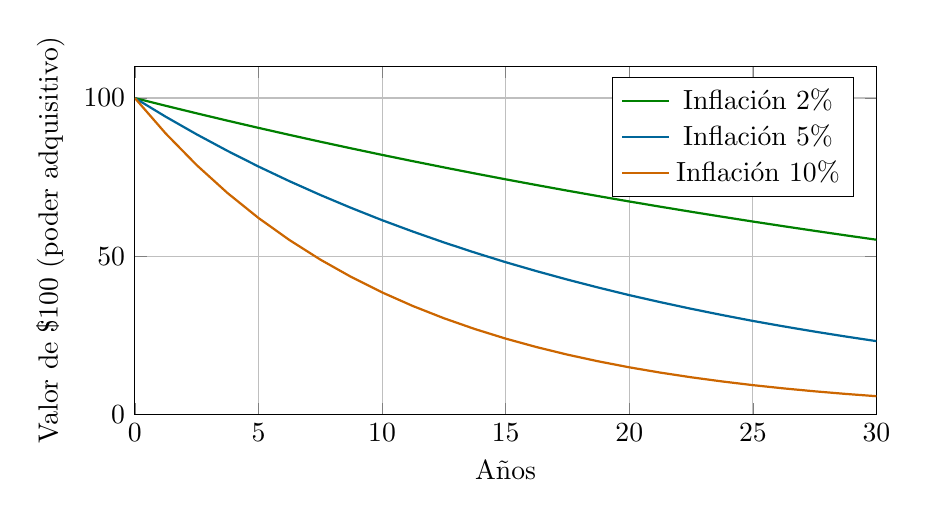
\begin{tikzpicture}
            \begin{axis}[
                xlabel={Años},
                ylabel={Valor de \$100 (poder adquisitivo)},
                xmin=0, xmax=30,
                ymin=0, ymax=110,
                grid=major,
                width=11cm,
                height=6cm,
                legend pos=north east
            ]
            % Inflación 2%
            \addplot[color=accentgreen, thick, domain=0:30] {100/(1.02)^x};
            \addlegendentry{Inflación 2\%}
            % Inflación 5%
            \addplot[color=primaryblue, thick, domain=0:30] {100/(1.05)^x};
            \addlegendentry{Inflación 5\%}
            % Inflación 10%
            \addplot[color=accentorange, thick, domain=0:30] {100/(1.10)^x};
            \addlegendentry{Inflación 10\%}
            \end{axis}
        \end{tikzpicture}
    \end{center}

    \textbf{Observación:} Al 5\% anual, \$100 pierden la mitad de su valor en $\approx$ 14 años.
\end{frame}

\begin{frame}{Tasa Nominal vs. Real vs. Inflación}
    \begin{center}
        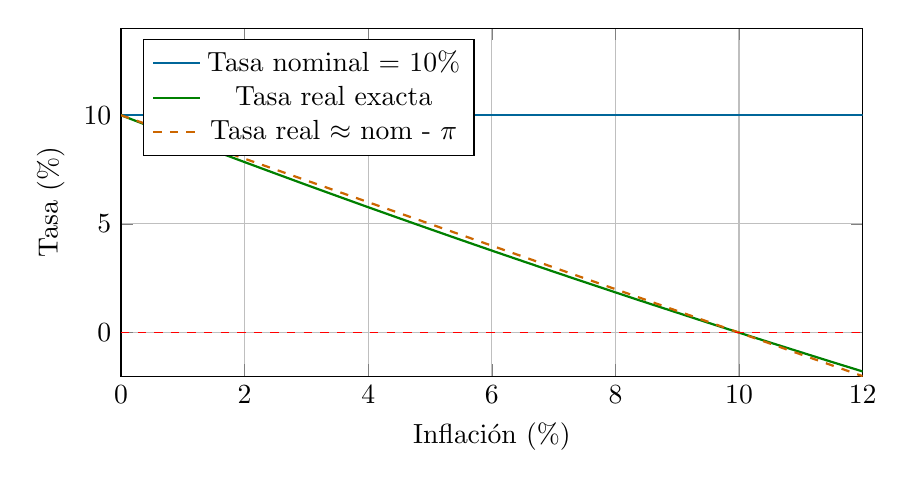
\begin{tikzpicture}
            \begin{axis}[
                xlabel={Inflación (\%)},
                ylabel={Tasa (\%)},
                xmin=0, xmax=12,
                ymin=-2, ymax=14,
                grid=major,
                width=11cm,
                height=6cm,
                legend pos=north west
            ]
            % Tasa nominal fija
            \addplot[color=primaryblue, thick, domain=0:12] {10};
            \addlegendentry{Tasa nominal = 10\%}
            % Tasa real exacta
            \addplot[color=accentgreen, thick, domain=0:12] {(1.10/(1+x/100) - 1)*100};
            \addlegendentry{Tasa real exacta}
            % Tasa real aproximada
            \addplot[color=accentorange, thick, dashed, domain=0:12] {10 - x};
            \addlegendentry{Tasa real $\approx$ nom - $\pi$}
            % Línea de tasa real = 0
            \addplot[color=red, dashed, domain=0:12] {0};
            \end{axis}
        \end{tikzpicture}
    \end{center}

    Cuando la inflación iguala la tasa nominal, la tasa real es cero.
\end{frame}

\begin{frame}{Crecimiento Nominal vs. Real}
    \textbf{Inversión de \$10,000 al 8\% nominal, inflación 5\%:}

    \begin{center}
        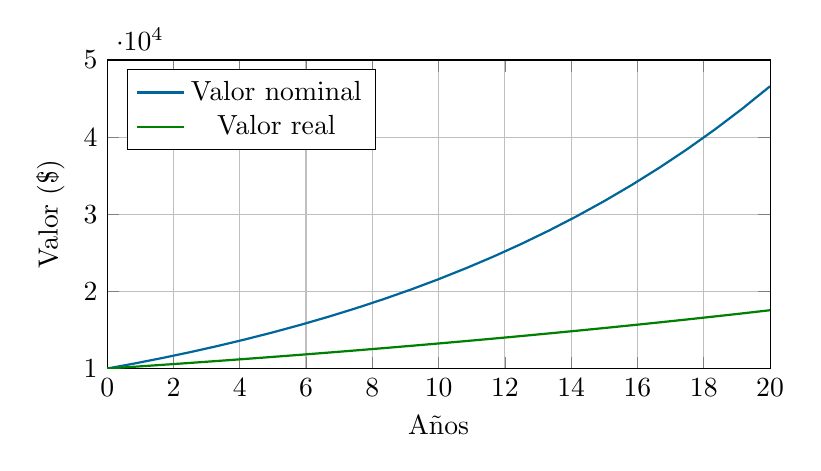
\begin{tikzpicture}
            \begin{axis}[
                xlabel={Años},
                ylabel={Valor (\$)},
                xmin=0, xmax=20,
                ymin=10000, ymax=50000,
                grid=major,
                width=10cm,
                height=5.5cm,
                legend pos=north west
            ]
            % Valor nominal
            \addplot[color=primaryblue, thick, domain=0:20] {10000*(1.08)^x};
            \addlegendentry{Valor nominal}
            % Valor real (en pesos de hoy)
            \addplot[color=accentgreen, thick, domain=0:20] {10000*(1.08/1.05)^x};
            \addlegendentry{Valor real}
            \end{axis}
        \end{tikzpicture}
    \end{center}

    En 20 años: Nominal = \$46,610, Real = \$17,536 (en poder adquisitivo de hoy).
\end{frame}

% ===========================================
% SECCIÓN 5: TRUCOS DE ESTIMACIÓN
% ===========================================
\section{Trucos de Estimación Mental}

\begin{frame}{Regla del 70 para Inflación}
    \begin{alertblock}{Regla del 70}
        Para estimar en cuántos años la inflación reduce el poder adquisitivo a la mitad:
        \[
        \boxed{n \approx \frac{70}{\pi\%}}
        \]
    \end{alertblock}

    \pause
    \vspace{0.5cm}

    \textbf{Ejemplos:}
    \begin{itemize}
        \item Inflación 2\%: $70/2 = 35$ años para perder la mitad
        \item Inflación 5\%: $70/5 = 14$ años para perder la mitad
        \item Inflación 10\%: $70/10 = 7$ años para perder la mitad
    \end{itemize}

    \pause
    \vspace{0.3cm}

    \begin{exampleblock}{Verificación}
        Al 5\%: $(1.05)^{14} = 1.98 \approx 2$ \checkmark
    \end{exampleblock}
\end{frame}

\begin{frame}{Aproximación de Fisher Mejorada}
    \begin{alertblock}{Para tasas moderadas}
        \[
        r_{real} \approx r_{nom} - \pi - \frac{r_{nom} \cdot \pi}{1 + \pi}
        \]
    \end{alertblock}

    \pause
    \vspace{0.3cm}

    \textbf{Ejemplo:} $r_{nom} = 15\%$, $\pi = 8\%$

    \pause
    \textbf{Aproximación simple:} $r_{real} \approx 15\% - 8\% = 7\%$

    \pause
    \textbf{Aproximación mejorada:}
    \begin{align*}
        r_{real} &\approx 15\% - 8\% - \frac{0.15 \times 0.08}{1.08} \\
        &= 7\% - 1.11\% = 5.89\%
    \end{align*}

    \pause
    \textbf{Exacto:} $\frac{1.15}{1.08} - 1 = 6.48\%$

    La aproximación mejorada es más precisa cuando las tasas son altas.
\end{frame}

\begin{frame}{Tabla de Referencia Rápida}
    \textbf{Tasa real aproximada ($r_{nom} - \pi$) vs. exacta:}

    \vspace{0.3cm}

    \begin{center}
    \begin{tabular}{@{}cc|cc|c@{}}
        \toprule
        $r_{nom}$ & $\pi$ & Aprox. & Exacta & Error \\
        \midrule
        5\% & 2\% & 3.00\% & 2.94\% & 0.06 pp \\
        8\% & 3\% & 5.00\% & 4.85\% & 0.15 pp \\
        10\% & 5\% & 5.00\% & 4.76\% & 0.24 pp \\
        15\% & 8\% & 7.00\% & 6.48\% & 0.52 pp \\
        20\% & 12\% & 8.00\% & 7.14\% & 0.86 pp \\
        30\% & 25\% & 5.00\% & 4.00\% & 1.00 pp \\
        \bottomrule
    \end{tabular}
    \end{center}

    \pause
    \vspace{0.3cm}

    \textbf{Conclusión:} La aproximación funciona bien para tasas bajas; usar la fórmula exacta cuando $\pi > 10\%$.
\end{frame}

% ===========================================
% SECCIÓN 6: HP 12C
% ===========================================
\section{Calculadora HP 12C}

\begin{frame}{HP 12C: Cálculo de Tasa Real}
    No hay función directa para tasa real, pero podemos calcularla paso a paso.

    \pause
    \vspace{0.3cm}

    \begin{block}{Problema}
        Calcular la tasa real si $r_{nom} = 12\%$ y $\pi = 5\%$.
    \end{block}

    \pause
    \vspace{0.3cm}

    \begin{center}
    \begin{tabular}{@{}lll@{}}
        \toprule
        \textbf{Teclas} & \textbf{Display} & \textbf{Descripción} \\
        \midrule
        \texttt{1.12 ENTER} & 1.12 & Factor nominal \\
        \texttt{1.05 $\div$} & 1.0667 & Factor real \\
        \texttt{1 -} & 0.0667 & Tasa real decimal \\
        \texttt{100 $\times$} & \textbf{6.67} & Tasa real \% \\
        \bottomrule
    \end{tabular}
    \end{center}

    \pause
    \vspace{0.3cm}

    \textbf{Tasa real = 6.67\%}
\end{frame}

\begin{frame}{HP 12C: Valor Presente con Inflación}
    \begin{block}{Problema}
        Recibirás \$50,000 nominales en 5 años. La tasa nominal es 10\% y la inflación 4\%. ¿Cuál es el VP?
    \end{block}

    \pause
    \vspace{0.3cm}

    \textbf{Opción 1: Usar tasa nominal directamente}
    \begin{center}
    \begin{tabular}{@{}lll@{}}
        \toprule
        \textbf{Teclas} & \textbf{Display} & \textbf{Descripción} \\
        \midrule
        \texttt{f CLX} & 0.00 & Limpiar \\
        \texttt{50000 FV} & 50,000.00 & Valor futuro nominal \\
        \texttt{10 i} & 10.00 & Tasa nominal \\
        \texttt{5 n} & 5.00 & Períodos \\
        \texttt{PV} & \textbf{-31,046.07} & Valor presente \\
        \bottomrule
    \end{tabular}
    \end{center}
\end{frame}

\begin{frame}{HP 12C: Poder Adquisitivo del VP}
    \textbf{Continuando el ejemplo anterior...}

    El VP de \$31,046 está en pesos de hoy. ¿Cuál es su poder adquisitivo en 5 años?

    \pause
    \vspace{0.3cm}

    \textbf{Ajuste por inflación futura:}
    \begin{center}
    \begin{tabular}{@{}lll@{}}
        \toprule
        \textbf{Teclas} & \textbf{Display} & \textbf{Descripción} \\
        \midrule
        \texttt{31046.07 PV} & 31,046.07 & VP calculado \\
        \texttt{4 i} & 4.00 & Tasa de inflación \\
        \texttt{5 n} & 5.00 & Períodos \\
        \texttt{FV} & \textbf{37,773.24} & Equivalente nominal en año 5 \\
        \bottomrule
    \end{tabular}
    \end{center}

    \pause
    \vspace{0.3cm}

    \$31,046 hoy tienen el mismo poder adquisitivo que \$37,773 en 5 años.
\end{frame}

% ===========================================
% SECCIÓN 7: EJERCICIOS PRÁCTICOS
% ===========================================
\section{Ejercicios Prácticos}

\begin{frame}{Ejercicio 1: Tasa Real Básica}
    \begin{block}{Problema}
        Un CETE paga 11\% anual nominal. La inflación esperada es 4.5\%. ¿Cuál es la tasa real esperada?
    \end{block}

    \pause
    \vspace{0.3cm}

    \textbf{Solución exacta:}
    \begin{align*}
        r_{real} &= \frac{1 + r_{nom}}{1 + \pi} - 1 \\
        r_{real} &= \frac{1.11}{1.045} - 1 \\
        r_{real} &= 1.0622 - 1 = 6.22\%
    \end{align*}

    \pause
    \vspace{0.2cm}

    \textbf{Aproximación:} $r_{real} \approx 11\% - 4.5\% = 6.5\%$

    \textbf{Error:} 0.28 pp (aceptable para estimaciones rápidas).
\end{frame}

\begin{frame}{Ejercicio 2: Tasa Nominal Requerida}
    \begin{block}{Problema}
        Un inversionista requiere un rendimiento real mínimo de 4\%. Si la inflación esperada es 6\%, ¿qué tasa nominal mínima debe exigir?
    \end{block}

    \pause
    \vspace{0.3cm}

    \textbf{Usando la ecuación de Fisher:}
    \begin{align*}
        (1 + r_{real})(1 + \pi) &= (1 + r_{nom}) \\
        (1.04)(1.06) &= 1 + r_{nom} \\
        1.1024 &= 1 + r_{nom} \\
        r_{nom} &= 10.24\%
    \end{align*}

    \pause
    \vspace{0.2cm}

    \textbf{Verificación con aproximación:} $r_{nom} \approx 4\% + 6\% = 10\%$ (cerca).

    \textbf{Respuesta:} Debe exigir al menos 10.24\% nominal.
\end{frame}

\begin{frame}{Ejercicio 3: Flujos Reales y Nominales}
    \begin{block}{Problema}
        Un proyecto genera \$100,000 reales anuales por 3 años. La tasa real de descuento es 5\% y la inflación es 3\%. Calcula el VP usando ambos métodos.
    \end{block}

    \pause
    \vspace{0.2cm}

    \textbf{Método Real:}
    \begin{align*}
        VP &= \frac{100,000}{1.05} + \frac{100,000}{(1.05)^2} + \frac{100,000}{(1.05)^3} \\
        VP &= 95,238 + 90,703 + 86,384 = \$272,325
    \end{align*}

    \pause
    \textbf{Método Nominal:} $r_{nom} = 1.05 \times 1.03 - 1 = 8.15\%$
    \begin{align*}
        CF_{1} &= 100,000 \times 1.03 = 103,000 \\
        CF_{2} &= 100,000 \times (1.03)^2 = 106,090 \\
        CF_{3} &= 100,000 \times (1.03)^3 = 109,273
    \end{align*}
    $VP = \frac{103,000}{1.0815} + \frac{106,090}{(1.0815)^2} + \frac{109,273}{(1.0815)^3} = \$272,324$
\end{frame}

\begin{frame}{Ejercicio 4: Planificación del Retiro}
    \begin{block}{Problema}
        Necesitas \$500,000 en poder adquisitivo de hoy para retirarte en 25 años. Si la inflación promedio será 3\% y puedes invertir al 7\% nominal, ¿cuánto debes invertir hoy?
    \end{block}

    \pause
    \vspace{0.3cm}

    \textbf{Paso 1:} Calcular cuánto necesitas nominalmente en 25 años:
    \begin{align*}
        F_{nom} = 500,000 \times (1.03)^{25} = 500,000 \times 2.0938 = \$1,046,900
    \end{align*}

    \pause
    \textbf{Paso 2:} Calcular VP con tasa nominal:
    \begin{align*}
        P = \frac{1,046,900}{(1.07)^{25}} = \frac{1,046,900}{5.4274} = \$192,912
    \end{align*}

    \pause
    \textbf{Respuesta:} Debes invertir \$192,912 hoy.
\end{frame}

\begin{frame}{Ejercicio 5: Comparación de Inversiones}
    \begin{block}{Problema}
        Inversión A: 9\% nominal garantizado. Inversión B: 4\% real garantizado (indexada). Si la inflación esperada es 4\% pero puede variar entre 2\% y 8\%, ¿cuál es mejor?
    \end{block}

    \pause
    \vspace{0.3cm}

    \textbf{Análisis:}
    \begin{center}
    \begin{tabular}{@{}ccc@{}}
        \toprule
        Inflación & $r_{real}$ de A & $r_{real}$ de B \\
        \midrule
        2\% & $(1.09/1.02)-1 = 6.86\%$ & 4\% \\
        4\% & $(1.09/1.04)-1 = 4.81\%$ & 4\% \\
        8\% & $(1.09/1.08)-1 = 0.93\%$ & 4\% \\
        \bottomrule
    \end{tabular}
    \end{center}

    \pause
    \vspace{0.3cm}

    \textbf{Conclusión:} A es mejor si la inflación es baja; B protege contra inflación alta.
\end{frame}

% ===========================================
% SECCIÓN 8: PYTHON
% ===========================================
\section{Python con numpy-financial}

\begin{frame}[fragile]{Python: Funciones para Tasas Reales}
    \begin{lstlisting}[style=pythonstyle]
import numpy as np

def tasa_real_exacta(r_nom, inflacion):
    """Calcula tasa real usando ecuacion de Fisher exacta."""
    return (1 + r_nom) / (1 + inflacion) - 1

def tasa_real_aprox(r_nom, inflacion):
    """Aproximacion simple de Fisher."""
    return r_nom - inflacion

def tasa_nominal_requerida(r_real, inflacion):
    """Calcula tasa nominal dada tasa real e inflacion."""
    return (1 + r_real) * (1 + inflacion) - 1

# Ejemplos
r_nom = 0.12
pi = 0.05

print(f"Tasa nominal: {r_nom*100:.2f}%")
print(f"Inflacion: {pi*100:.2f}%")
print(f"Tasa real (exacta): {tasa_real_exacta(r_nom, pi)*100:.2f}%")
print(f"Tasa real (aprox): {tasa_real_aprox(r_nom, pi)*100:.2f}%")
    \end{lstlisting}
\end{frame}

\begin{frame}[fragile]{Python: Valor Presente con Inflación}
    \begin{lstlisting}[style=pythonstyle]
import numpy_financial as npf

def vp_flujos_reales(flujos_reales, r_real):
    """VP de flujos reales con tasa real."""
    vp = 0
    for t, cf in enumerate(flujos_reales):
        if t > 0:  # flujo en periodo t
            vp += cf / (1 + r_real)**t
    return vp

def vp_flujos_nominales(flujos_reales, r_nom, inflacion):
    """VP de flujos convertidos a nominales."""
    vp = 0
    for t, cf in enumerate(flujos_reales):
        if t > 0:
            cf_nom = cf * (1 + inflacion)**t
            vp += cf_nom / (1 + r_nom)**t
    return vp

flujos = [0, 100000, 100000, 100000]  # 100k reales por 3 años
print(f"VP (metodo real): ${vp_flujos_reales(flujos, 0.05):,.2f}")
print(f"VP (metodo nominal): ${vp_flujos_nominales(flujos, 0.0815, 0.03):,.2f}")
    \end{lstlisting}
\end{frame}

\begin{frame}[fragile]{Python: Simulación de Poder Adquisitivo}
    \begin{lstlisting}[style=pythonstyle]
import matplotlib.pyplot as plt
import numpy as np

años = np.arange(0, 31)
inversion_inicial = 100000
r_nom = 0.08
inflacion = 0.05

# Valor nominal
valor_nominal = inversion_inicial * (1 + r_nom)**años

# Valor real (poder adquisitivo)
valor_real = valor_nominal / (1 + inflacion)**años

plt.figure(figsize=(10, 6))
plt.plot(años, valor_nominal/1000, 'b-', label='Valor Nominal')
plt.plot(años, valor_real/1000, 'g-', label='Valor Real')
plt.xlabel('Años')
plt.ylabel('Valor (miles de $)')
plt.title('Crecimiento Nominal vs Real')
plt.legend()
plt.grid(True)
plt.savefig('nominal_vs_real.png')
    \end{lstlisting}
\end{frame}

% ===========================================
% SECCIÓN 9: RESUMEN Y TAREA
% ===========================================
\section{Resumen y Tarea}

\begin{frame}{Resumen de Fórmulas}
    \begin{columns}
        \begin{column}{0.5\textwidth}
            \textbf{Ecuación de Fisher}
            \[
            (1 + r_{real})(1 + \pi) = (1 + r_{nom})
            \]

            \textbf{Tasa Real Exacta}
            \[
            r_{real} = \frac{1 + r_{nom}}{1 + \pi} - 1
            \]

            \textbf{Aproximación}
            \[
            r_{real} \approx r_{nom} - \pi
            \]
        \end{column}

        \begin{column}{0.5\textwidth}
            \textbf{Flujos Nominales}
            \[
            CF_{nom,t} = CF_{real} \times (1 + \pi)^t
            \]

            \textbf{Regla del 70}
            \[
            n_{\div 2} \approx \frac{70}{\pi\%}
            \]

            \textbf{Tasa Nominal Requerida}
            \[
            r_{nom} = (1+r_{real})(1+\pi) - 1
            \]
        \end{column}
    \end{columns}
\end{frame}

\begin{frame}{Conceptos Clave}
    \begin{enumerate}
        \item La \textbf{inflación} erosiona el poder adquisitivo del dinero
        \item La \textbf{tasa real} mide el verdadero rendimiento ajustado
        \item La \textbf{ecuación de Fisher} relaciona tasas nominales, reales e inflación
        \item Flujos nominales $\to$ tasa nominal; Flujos reales $\to$ tasa real
        \item Los \textbf{instrumentos indexados} protegen contra la inflación
        \item Las tasas reales pueden ser \textbf{negativas}
        \item La \textbf{Regla del 70} estima el tiempo para perder la mitad del valor
    \end{enumerate}
\end{frame}

\begin{frame}{Tarea para la Próxima Sesión}
    \begin{enumerate}
        \item \textbf{Ejercicios HP 12C:}
        \begin{itemize}
            \item Calcular tasa real si $r_{nom} = 15\%$ y $\pi = 9\%$
            \item VP de \$200,000 nominales en 10 años, $r_{nom} = 8\%$, $\pi = 3\%$
        \end{itemize}

        \vspace{0.3cm}

        \item \textbf{Problema:} Un bono paga \$1,000 reales anuales por 5 años. Si $r_{real} = 3\%$ y $\pi = 4\%$, calcula el VP usando ambos métodos.

        \vspace{0.3cm}

        \item \textbf{Python:} Grafica cómo cambia la tasa real cuando la inflación varía de 0\% a 15\%, manteniendo $r_{nom} = 10\%$ fijo.

        \vspace{0.3cm}

        \item \textbf{Investigación:} Busca la inflación actual de tu país y calcula la tasa real de una cuenta de ahorro típica.
    \end{enumerate}
\end{frame}

% ===========================================
% CIERRE
% ===========================================

\begin{frame}
    \begin{center}
        \Huge \textcolor{primaryblue}{\textbf{¿Preguntas?}}

        \vspace{1cm}
        \Large Próxima Sesión:\\
        \textbf{Anualidades Ordinarias (Vencidas)}

        \vspace{0.5cm}
        \normalsize Semana 3, Clase 1
    \end{center}
\end{frame}

\end{document}
